\PassOptionsToPackage{top=3cm,left=3cm,right=3cm,bottom=3cm}{geometry}
\documentclass[fleqn,11pt]{wlscirep}

\usepackage{import}
\usepackage{main-lancet}

\renewcommand{\paragraph}[1]{\vspace{0.3cm}\noindent\underline{\emph{#1}}\hfill\noindent}

% word count
% \newcommand{\maincount}[1]{%
%   \immediate\write18{texcount -1 -sum=1 -merge -q -nobib #1.tex > #1-words.sum}%
%   \input{#1-words.sum}%
% }

% \newcommand{\abstractcount}[1]{%
%   \immediate\write18{texcount -template="{abst}" #1.tex > #1-words.sum}%
%   \input{#1-words.sum}%
% }

\begin{document}

\doublespacing

\title{\bfseries\LARGE\singlespacing{Impact of air cleaners in schoolson respiratory viral infections: A modeling study using epidemiological, environmental, and molecular data}}

% Alternative title: SARS-CoV-2 transmission in schools based on molecular and epidemiological data: potential effects of mask wearing and air cleaners

% author list
\author[1$\ddag$,2]{Nicolas Banholzer}
\author[2,3]{Philipp Jent}
\author[2,4]{Pascal Bittel}
\author[1]{Kathrin Zürcher}
\author[4]{Lavinia Furrer}
\author[1]{Simon Bertschinger}
\author[5]{Ernest Weingartner}
\author[2,4]{Alban Ramette}
\author[2,4]{Ronald Dijkman}
\author[1]{Matthias Egger}
\author[6]{Tina Hascher}
\author[1*,2]{Lukas Fenner}

\affil[1]{Institute of Social and Preventive Medicine, University of Bern, Bern, Switzerland}
\affil[2]{Multidisciplinary Center for Infectious Diseases, University of Bern, Bern, Switzerland}
\affil[3]{Department of Infectious Diseases, Inselspital, Bern University Hospital, University of Bern, Bern, Switzerland}
\affil[4]{Institute for Infectious Diseases, University of Bern, Bern, Switzerland}
\affil[5]{School of Engineering, University of Applied Sciences and Arts Northwestern Switzerland, Windisch, Switzerland}
\affil[6]{Institute of Educational Science, University of Bern, Bern, Switzerland}


\affil[*]{Corresponding author: lukas.fenner@unibe.ch }


\vspace{1em}

\begin{information}\normalfont

\noindent \textcolor{red}{[list of appendices to be added here later; including STROBE]}

% \noindent\textbf{S1 Appendix:} Includes supplementary text, tables and figures.


% \par
\end{information}

%TC:ignore
\begin{abstract}\normalfont
\noindent\textbf{Background:} Infection control measures can reduce airborne transmission. Using a multiple-measurement approach, we aimed to evaluate the real-world effectiveness of portable HEPA-air filtration devices (air cleaners) in reducing transmission of respiratory viral infections in schools. \medskip

\noindent\textbf{Methods:} We collected epidemiological data (absences related to respiratory infections), environmental data (CO$_2$ and particle concentrations), audio recordings (coughing), and molecular data (bioaerosol and saliva samples) over seven weeks during winter 2023 in two classes of a Swiss secondary school. Using a cross-over study design, we compared particle concentrations, coughing, and the risk of infection with and without air cleaners.  \medskip

\noindent\textbf{Results:} Molecular analysis detected multiple viruses in saliva (50/448 positive: 15~influenza B, 15~rhinovirus, 14~adenovirus, 3~SARS-CoV-2, 2~metapneumovirus, and 1~parainfluenza), but rarely in bioaerosol samples (2/105 positive) and on the filters of air cleaners (4/160~positive). Spatiotemporal analysis of positive saliva samples suggested within-classroom transmission. Testing positive was equally likely with air cleaners (adjusted relative risk [ARR] 0.93 95\%-credible interval [CrI] 0.49 to 1.61). CO$_2$ levels were similar (1,769$\pm$391\,ppm with vs. 1,636$\pm$341\,ppm without air cleaners), yet particle concentrations decreased by 77\%, (95\%-CrI 63\% to 86\%) and coughing was slightly less frequent (ARR 0.93, 95\%-CrI 0.85 to 1.02). Infection risk was also lower (posterior probability 91\%), but the association was small (ARR 0.72, 95\%-CrI 0.44 to 1.15). \medskip 

\noindent\textbf{Conclusions:} A wide range of non-SARS-CoV-2 respiratory viruses were detected in student saliva. Although airborne detection was rare, transmission seemed likely in schools, suggesting that prolonged close contact is required for transmission. Air cleaners improved air quality, were associated with lower symptom intensity, and showed a potential benefit in reducing infections.

\par
\end{abstract}

\flushbottom
\maketitle

\vspace{2em}

\vspace{0.5em}

\noindent\textbf{Keywords:} schools, air cleaner, respiratory viruses, airborne transmission, molecular detection
% maximum of 3-5 keywords

\thispagestyle{empty}
\sloppy
\raggedbottom

\newpage

\noindent\textbf{\Large{Research in context}} \medskip

\noindent \textbf{Evidence before this study} \smallskip

\noindent \textcolor{red}{[Search and search terms to be added]} Several studies have shown that air cleaners reduce particle concentrations in indoor air. Another study showed that air cleaners effectively removed SARS-CoV-2 bioaerosols in a hospital ward. A simulation studies have demonstrated the efficacy of air cleaners in reducing the risk of indoor transmission. A real-world study during the pandemic showed a trend toward a reduction of the infection risk. \medskip

\noindent \textbf{Added value of this study} \smallskip

\noindent We showed the transmission dynamics in classrooms of a secondary school under non-pandemic conditions. Although airborne detection was rare, transmission seemed likely in schools, suggesting that prolonged close contact is required for transmission. Air cleaners improved air quality, were associated with lower symptom intensity, and showed a small, potential benefit in reducing infections.\medskip

\noindent \textbf{Implications of all the available evidence} \smallskip

\noindent Good ventilation improves indoor air quality and can reduce the risk of infection under non-pandemic conditions. Greater emphasis should be given to ventilation systems in schools in the long term. Seasonal respiratory viruses other than SARS-CoV-2 may require prolonged close contact. Future studies should examine the relative importance of prolonged close contact and long-distance transmission of respiratory viruses in schools and other congregate settings.

\thispagestyle{empty}
\sloppy
\raggedbottom

\newpage
%TC:endignore

\setcounter{page}{1}

\section{Introduction} 

Transmission of respiratory infections such as SARS-CoV-2 and influenza are difficult to mitigate and control. Person-to-person transmission occurs primarily through the release of respiratory particles containing the viruses. Recent focus has been on small respiratory particles called aerosols ($\leq$ 5$\mu$m), which have been found to carry the majority of viruses during respiratory activities\cite{Fennelly2020}. Unlike larger respiratory droplets, which tend to settle quickly, aerosols can remain suspended in the air for several hours and travel long distances\cite{Coleman2022,Wang2020,Heneghan2021}.

Improved ventilation systems are critical for a healthy indoor environment and can reduce the risk of respiratory transmission\cite{Wang2021,Morawska2021}. Portable HEPA-air filtration devices (air cleaners) may be another cost-effective alternative to upgrading ventilation systems. Still, the effects of air cleaners on the transmission of respiratory infections are less clear. Several studies have shown that air cleaners reduce particle concentrations in indoor air\cite{Park2020Build,Buising2022InfContr,Banholzer2023PLoSMed}, which is associated with a reduced risk of respiratory infection and mortality\cite{Gordon2014Resp,Kelly2023Atmos,DeAngelis2021EnvRes}. In addition, a recent study showed that air cleaners effectively removed SARS-CoV-2 bioaerosols in a hospital ward\cite{Morris2022}. Simulation studies have demonstrated the efficacy of air cleaners in reducing the risk of indoor transmission  of SARS-CoV-2\cite{Lindsley2021} and other respiratory viruses\cite{Cortellessa2023Build}. To date, it remains unclear whether reducing particle concentrations and removing bioaerosols from the air will reduce transmission of respiratory infections. 

We used a multiple-measurement approach to study the transmission of respiratory viruses under non-pandemic conditions and the effect of air cleaners in schools with a cross-over study design in the winter of 2023. We collected epidemiological data (absences likely related to respiratory infections), environmental data (CO$_2$, particle concentrations), audio recordings (coughing), and molecular data (detection of viruses in bioaerosol and human saliva samples) during a seven-week study period from January to March 2022 in two classes of a secondary school in Switzerland. We determined changes in absences related to respiratory infections, positivity rates of saliva samples, particle concentrations, and coughing.

\newpage

\section{Methods}

\subsection{Study setting and design} 

\noindent We collected data in two classrooms of a secondary school (age of students 14-17~years) in the canton of Solothurn, Switzerland, for seven weeks from January~16 to March~11, 2023. Figure~\ref{fig:study-setup} shows the schematic study setup, and \supp~table~\zref{tab:data} provides an overview of the types of data collected.

\begin{figure}[!htpb]
    \centering
    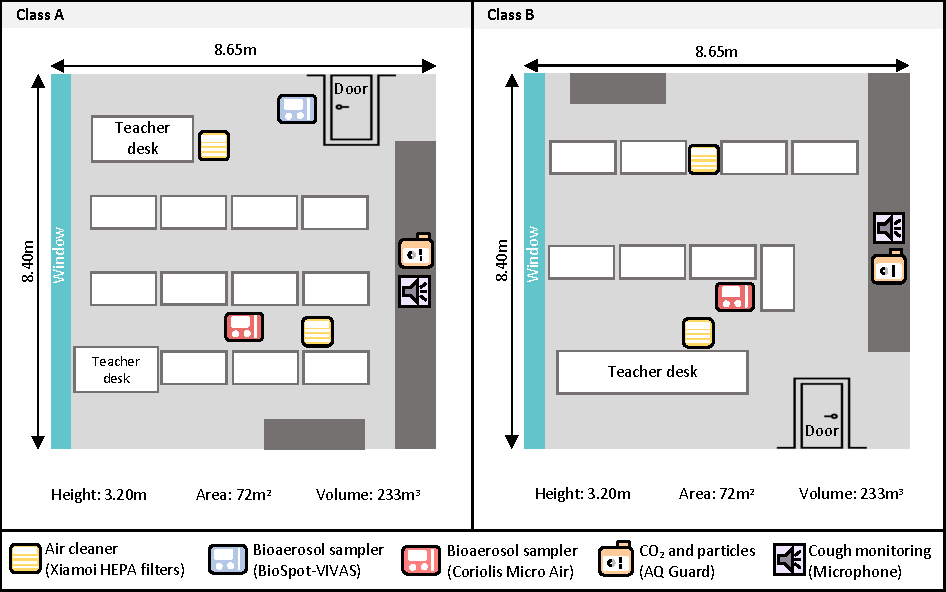
\includegraphics{../study_setting.pdf}
    \caption{\textbf{Study setting}. Schematic study setup of the classrooms. One air cleaner was placed in the front and one in the back of the classrooms. All devices were placed at the head level of the students when they were seated. Neither classrooms was equipped with an active HVAC (Heating, Ventilation, Air conditioning) system, but they were ventilated naturally by opening windows. }
    \label{fig:study-setup}
\end{figure}

\subsection{Study intervention} 

\noindent We used a cross-over design to study the effectiveness of air cleaners, with two study conditions: weeks with and weeks without air cleaners being installed in each classroom (\cref{tab:study_design}). Air cleaners refer to commercially available portable HEPA-filtration devices (Xiaomi Mi Air Pro 70m², Shenzhen, China). According to the manufacturer, these air cleaners run at clean air delivery rates of 2$\,\times\,$600 m$^{3}$/h. Window ventilation was done at the discretion of the teachers, as there were no specific recommendations from the national health authorities at the time.

\begin{table}[!htpb]
    \footnotesize
    \centering
    \caption{\textbf{Study design.} Cross-over design describing when portable air cleaners (AC) were installed in the rooms of classes A and B during a seven-week study period from January~16 to March~11, 2023, excluding a week of vacation from February 6 to 11.}\label{tab:study_design}
    \begin{tabular}{l l l l l l l l l}
    \toprule
      & \textbf{Week 1} & \textbf{Week 2} & \textbf{Week 3} & Vacation & \textbf{Week 4} & \textbf{Week 5} & \textbf{Week 6} & \textbf{Week 7} \\
      & Jan 16-21 & Jan 23-28 & Jan 30-Feb 3 & Feb 6-11 & Feb 13-18 & Feb 20-25 & Feb 27-Mar 3 & Mar 6-11 \\
      \midrule
      \textbf{A} & \cellcolor{gray!50} AC & \cellcolor{gray!50} AC\hphantom{0000}*& \cellcolor{gray!10} None & & \cellcolor{gray!10} None & \cellcolor{gray!10} None & \cellcolor{gray!50} AC & \cellcolor{gray!50} AC\hphantom{00009}* \\
      \textbf{B} & \cellcolor{gray!10} None & \cellcolor{gray!10} None & \cellcolor{gray!50} AC\hphantom{0000000}* & & \cellcolor{gray!50} AC & \cellcolor{gray!50} AC\hphantom{0000}*& \cellcolor{gray!10} None & \cellcolor{gray!10} None \\
      \bottomrule
      \multicolumn{9}{l}{\scriptsize *~Swabs from the HEPA filters taken after each intervention phase and before the vacation.}
    \end{tabular}
\end{table}
 
\subsection{Data collection}

\noindent\textbf{Epidemiological data} \smallskip

\noindent At the beginning of the study, we collected aggregated data on age, sex, COVID-19 vaccination, and COVID-19 recovery status in the participating classes. Daily, we collected data on each absent student, \ie the absence and return dates and reason for the absence (illness, career days, or other). For absences due to illness, we recorded symptoms and the date of symptom onset. We defined a case of respiratory infection as an absence in which the student reported an illness with at least one respiratory symptom (\supp~text~\zref{sec:case-data}). The line list data is shown in \supp~table~\zref{tab:epi-data-line-list}. \medskip

\noindent\textbf{Molecular data} \smallskip

\noindent Both classes participated in repetitive bi-weekly testing (Tuesdays and Thursdays; see \nameref{sec:mol_analyses} below). Saliva samples were transported to the laboratory and stored at $-$80°C until further processing\cite{Galar2021,To2019,Huber2021}. The line list data is shown in \supp~table~\zref{tab:mol-data-line-list}. Furthermore, We collected airborne respiratory viruses in both classrooms with a bioaerosol sampling device (Coriolis Micro Air, Bertin Instruments Montigny-le-Bretonneux, France), running at 200\,l/min and collecting into 15\,mL Phosphate-Buffered Saline (PBS). The Coriolis Micro Air ran shortly before and during break times to prevent unacceptable noise exposure (approximately 60\,min/day). In one class, we also used the BioSpot-VIVAS device sampler (Aerosol Devices Inc., Ft. Collins, CO, USA) \cite{Pan2016JAM,Lednicky2016AST}. BioSpot-VIVAS operated throughout the lessons. The removable parts of both sampling devices were regularly autoclaved. At the end of the day, samples were transported to the Institute of Infectious Diseases (IFIK) and stored at $-$80°C. Finally, we collected swabs from the HEPA filters of the air cleaners after each intervention phase (see \cref{tab:study_design}). The HEPA filters were removed from the air cleaners and divided into 20~fields. One swab per field was then taken for a total of 20~swabs per filter. \medskip

\noindent\textbf{Environmental data} \smallskip

\noindent An air quality device (AQ Guard, Palas GmbH, Karlsruhe, Germany) continuously measured indoor CO$_2$ levels, aerosol number concentrations (particle diameter between 175~nm to 20~$\mu$m) and particle mass concentrations (PM; PM$_1$, PM$_{2.5}$, PM$_4$, PM$_{10}$) by minute. This device was used in previous work\cite{DiGilio2021,Duill2021,Banholzer2023PLoSMed}. 

\subsection{Laboratory and molecular analyses}\label{sec:mol_analyses}

\noindent Prior to the real-time (RT)-PCR analysis, daily bioaerosol samples were combined for each sampling device and filtered using Amicon Ultra-15 Centrifugal Filters with Ultracel 10,000 Dalton molecular weight cutoffs filters (UFC9010; MilliporeSigma, Burlington, USA) to a volume of 1\,mL. The human saliva samples were analyzed directly without prior filtration. The Allplex RV Master Assay (Seegene, Seoul, South Korea) detects a panel of 8~respiratory viruses, including SARS-CoV-2 (CoV), influenza (IF), respiratory syncytial (RSV), metapneumovirus (MPV), adenovirus (AdV), rhinovirus (HRV), and parainfluenza (PIV). 

\subsection{Molecular genotyping}

We performed molecular genotyping for positive saliva, bioaerosol, air filter samples of AdV and IF. For AdV, we used a PCR procedure to amplify three hypervariable regions of the viral genome and then sequenced the PCR products\cite{Akello2021SciRep}. For IF, we tried to determine the molecular transmission network using whole genome sequencing\cite{Kelly2022FrontiersImmuno}.

\subsection{Cough detection}

We installed a portable audio recorder (ZOOM H6; New York, USA) in each classroom to record sounds continuously. We determined the number of coughs per minute using an AI algorithm\cite{Bertschinger2023IEEE}.

\subsection{Statistical analyses and modeling}

All statistical analyses were described in the statistical analysis plan (SAP)\cite{Banholzer2023SAP}, which was published prior to the analyses. Contrary to the SAP, bioaerosol samples and viral load concentrations could not be analyzed because there were too few positive samples. Otherwise, there were no major deviations from the SAP. Minor deviations are documented in \supp~text~\zref{sec:transmission-model}-\zref{sec:env-regression-model}, including detailed descriptions of the models. \medskip

\noindent\textbf{Risk of infection} \smallskip

\noindent We estimated the relative risk of infection with air cleaners using a Bayesian latent variable hierarchical regression model. The observed outcome of this model is the number of new respiratory cases $C$ (absences related to respiratory infections by date of symptom onset) on day $t$ in class $j$, which are modeled with a Negative Binomial distribution. The expected number of new cases is the weighted sum of the number of new infections $I_{js}$ (unobserved/latent outcome) in the previous days $s<t$, with the weights corresponding to the probability distribution of the incubation period. The number of new infections is related to the presence of air cleaners using a regression-like log-link
\begin{align}
    \log I_{js} = \log F_{js} - \log N_{js} + \beta_0 + \beta_1 \cdot \text{AirCleaner}_{js},
\end{align}
where $F_{js}$ is the number of infections in the previous week (a proxy for the number of infectious students), $N_{js}$ is the cumulative number of infections (a proxy for the number of susceptible students), $\beta_0$ is the infection rate without air cleaners, and $\beta_1$ is the effect of air cleaners. Furthermore, the effect of air cleaners is adjusted for class-specific effects, the number of students in class, the daily air change rate, and the weekly positivity rate for COVID-19 and the consultations for influenza-like illnesses in the community (\ie the canton of Solothurn). A detailed description of the model and choice of priors for all model parameters are provided in \supp~text~\zref{sec:transmission-model}. 

\noindent\textbf{Number of positive saliva samples} \smallskip

\noindent We analyzed the number of positive saliva samples with a Bayesian Multinomial logistic regression model (\supp~text~\zref{sec:multinomial-model}) and linked the expected number of positive samples to the presence of air cleaners, adjusting for the cumulative number of positive tests.

\noindent\textbf{Aerosol and particle concentrations} \smallskip

\noindent We computed the average particle concentrations per day and compared them between study conditions. We estimated the reduction in particle concentrations using Bayesian log-linear regression models, adjusting for class and weekday effects, the number of students in class, the air change rate, and the cumulative number of respiratory cases (\supp~text~\zref{sec:env-regression-model}). \medskip

\noindent\textbf{Number of coughs} \smallskip

\noindent We computed the daily number of detected coughs and compared it between study conditions. We estimated the reduction in the number of coughs using a Bayesian Negative Binomial regression model, using time in class as the model offset and adjusting for class and weekday effects, the number of students in class, the air change rate, and the cumulative number of respiratory cases (\supp~text~\zref{sec:aud-regression-model}). In addition, we used a Bayesian Negative Binomial hierarchical (random effects) regression model to estimate the association between the number of coughs and the number of positive saliva test results. For this analysis, we used only days on which saliva samples were collected (Tuesdays and Thursdays, for a total of 27~days).  \medskip

\noindent\textbf{Software} \smallskip

\noindent All analyses were performed in R software (version 4.2.0)\cite{RCoreTeam2022} and modeling in Stan (version 2.21.0)\cite{Carpenter2017}. Model parameters were estimated with a Bayesian approach, using the Hamiltonian Monte Carlo algorithm with the No-U-Turn Sampler (NUTS)\cite{Hoffman2014}. If not stated otherwise, we report for each outcome the posterior probability (PP) that the adjusted relative risk (ARR) was lower with air cleaners (ARR<1). ARR is reported with mean and 95\%credible interval (CrI) based on 4,000 samples from the posterior distribution of each model. The code is available from \url{https://osf.io/38j9g}.


\subsection{Ethics statement}

\noindent The Ethics Committee of the canton of Bern, Switzerland, approved the study (reference no. 2021-02377). For the saliva samples, we included all students who were willing to participate and obtained written informed consent from their caregivers.


\newpage

\section{Results}

The study population consisted of 38~students (19~female, 19~male; Table~\ref{tab:cases-overview-school}). Seven~students had been vaccinated or recovered from a SARS-CoV-2 infection within the last four months. During the seven-week study period (total of 1,330 student-days), students were absent from school for 220~days (18\% of the total) of which 129~days (59\% of absences) were due to illness.  

\begin{table}[!htpb]
    \centering
    \caption{Overview of the study population and person-days of absences.}
    \label{tab:cases-overview-school}
    \footnotesize
    \renewcommand{\arraystretch}{1.5}
    \begin{tabular}{l r r r}
    \toprule
         &  Class A & Class B & Total \\ \midrule 
        \textbf{Students} & \textbf{20 (53\%)} & \textbf{18 (47\%)} & \textbf{38 (100\%)} \\
        \emph{Gender} \\
        $\drsh$ Female & 11 (55\%) & 8 (44\%) & 19 (\hphantom{0}50\%) \\
        $\drsh$ Male & 9 (45\%) & 10 (56\%) & 19 (\hphantom{0}50\%) \\
        \emph{Immunity status} \\
        $\drsh$ Recently vaccinated (or recovered) & 7 (39\%) & 0 (0\%) & 7 (\hphantom{0}18\%) \\
        $\drsh$ Not recently vaccinated (or recovered) & 11 (61\%) & 20 (100\%) & 31 (\hphantom{0}82\%) \\
        \textbf{Absent person-days} & \textbf{110 (50\%)} & \textbf{110 (50\%)} & \textbf{220 (100\%)} \\
        $\drsh$ Sickness & 52 (47\%) & 77 (70\%) & 129 (\hphantom{0}59\%) \\
        $\drsh$ Other & 58 (53\%) & 33 (30\%) & 91 (\hphantom{0}41\%) \\
        \bottomrule
    \end{tabular} 
\end{table}

\subsection{Molecular analyses of saliva and air samples}

We analyzed a total of 448~saliva samples. We detected 15~influenza~B~(Flu B), 15~rhinoviruses~(HRV), 14~adenoviruses (AdV), 3~SARS-CoV-2~(CoV), 2~metapneumoviruses~(MPV), and 1~parainfluenza~viruses~(PIV) (\cref{fig:molecular-descriptives}a). The distribution of positive saliva samples varied between classes. For example, during the first three study weeks, all but one sample was positive for AdV in class~A, while the vast majority of positive IFB samples were found in class~B. To illustrate possible transmission chains within classes, we linked positive saliva samples of the same virus that were less than one week apart. Based on this spatiotemporal analysis, we identified 10~possible transmission chains (\cref{fig:molecular-descriptives}b). The longest potential transmission chains occurred in January, referring to a cluster of AdV infections in class~A and IFB infections in class~B. 

Molecular genotyping to verify the proposed transmission network was unsuccessful because we could not amplify and sequence any of the gene targets. Furthermore, the rate of positive bioaerosol samples was low. We analyzed 105~bioaerosol samples and detected only two respiratory viruses in the air (1~HRV in class~A and 1~AdV in class~B). Similarly, we detected only 1~IFB, 1~HRV, 1~AdV, and 1~CoV in the 20~swabs taken from each filter of an air cleaner after each intervention phase (160~swabs in total). However, the virus-specific variation between classes and the temporal distribution of positive samples still suggest that transmission occurred within classes. 


\begin{figure}[!htpb]
    \centering
    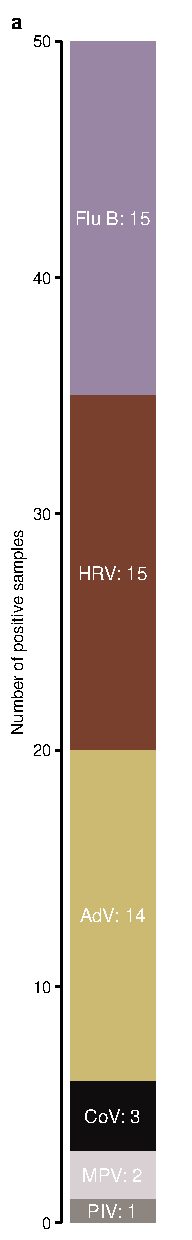
\includegraphics{../../results/mol-data/saliva-distribution.pdf}\hspace{.5cm}
    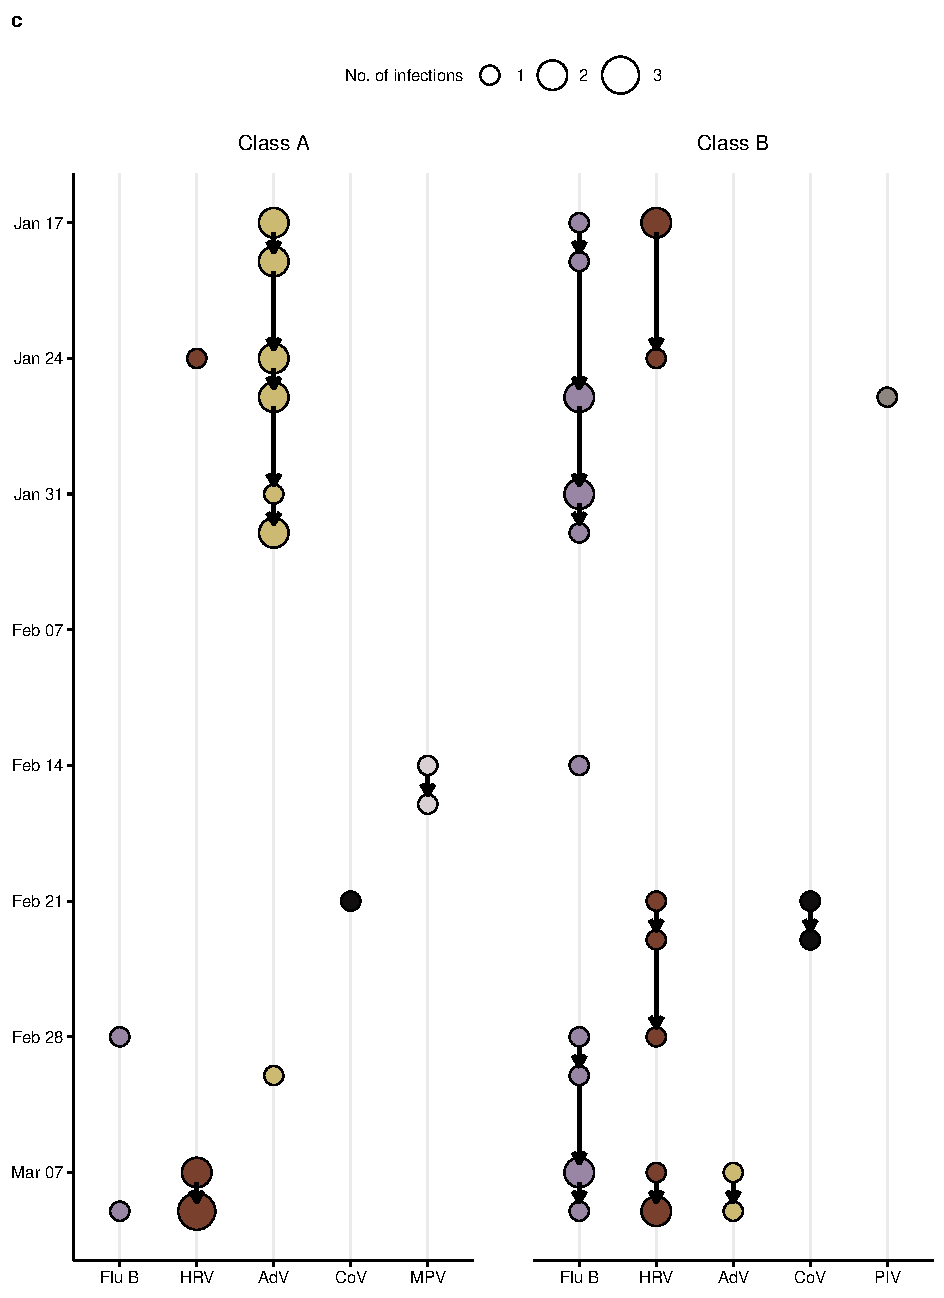
\includegraphics{../../results/mol-data/network-plot.pdf}
    \caption{\textbf{Molecular detection of respiratory viruses and transmission network based on spatiotemporal analysis of students' saliva samples}. \textbf{(a)}~Number of positive saliva samples by virus. \textbf{(b)}~Daily number of positive saliva samples (colored circles) and possible transmission chains within classes (directed arrows). Positive samples are linked if they belong to the same virus and are less than 1~week apart. Positive samples from the air and filters as blank squares aligned. Flu B: Influenza B, HRV: rhinovirus, AdV: adenovirus, CoV: SARS-CoV-2, MPV: metapneumovirus, PIV: parainfluenza virus.}
    \label{fig:molecular-descriptives}
\end{figure}

\subsection{Risk of infection with and without air cleaners}

There was an equal number of 25~positive saliva samples in both study conditions (\cref{fig:infection-risk}b). Based on our Bayesian Multinomial logistic regression model, the positivity rate remained comparable between study conditions (ARR 0.93, 95\%-CrI 0.49 to 1.61; PP 61\%). The estimated ARR was not sensitive to infection to testing delays (\supp~figure~\zref{fig:mol-estimation-results-sensitivity}).

The aerosol number concentration was 95$\pm$81\,1/cm$^3$ without and 27$\pm$34\,1/cm$^3$ with air cleaners (\cref{fig:infection-risk}a). The adjusted decrease in the aerosol concentration with air cleaners was 76\% (95\%-CrI 63\% to 86\%; PP 100\%). This decrease was greater for larger (PM$_{10}$) than for smaller (PM$_1$ to PM$_{4}$) particle matter mass concentrations  (\supp~figure~\zref{fig:palas-results} and \supp~table~\zref{tab:palas-est-results}). There was little change in other environmental variables (\supp~figure~\zref{fig:env-descriptives-other-vars}). In particular, daily average CO$_2$ levels were 1,769$\pm$391\,ppm with and 1,636$\pm$341\,ppm without air cleaners, suggesting that ventilation was comparable between study conditions.

Absences related to respiratory infections were 22~respiratory cases without and 13~cases with air cleaners (\cref{fig:infection-risk}c). Our Bayesian latent variable hierarchical regression model suggested that air cleaners reduced the risk of infection (PP 91\%). However, the reduction was small and subject to uncertainty (ARR 0.72, 95\%-CrI 0.44 to 1.15). The estimated number of infections would be 36 (95\%-CrI 21 to 64) if air cleaners had been installed throughout the study period, compared to 62 (95\%-CrI 29 to 141) infections if air cleaners had not been installed (\supp~\zref{fig:avoided-infections}). Detailed estimations are provided in the \supp~text~\zref{sec:detailed-redcap}. 

We detected 3.1$\pm$1.2~coughs/min in audio recordings without and 2.6$\pm$1.1~coughs/min with air cleaners (\cref{fig:infection-risk}d). Based on our Bayesian Negative Binomial regression model, the risk of coughing was slightly lower with air cleaners (ARR 0.93, 95\%-CrI 0.85 to 1.02; PP 93\%). Significantly more coughs were detected in the room of class~B (ARR 2.16, 95\%-CrI 1.90 to 2.46), suggesting an association with the observed variation in virus-specific transmission between classes. Indeed, cough was more frequent with IFB positivity (ARR 1.25, 95\%-CrI 1.03 to 1.53) and slightly less frequent with AdV positivity (ARR 0.87, 95\%-CrI 0.49 to 1.12) (\supp~figure~\zref{fig:coughing-association}b). 

\begin{figure}[!htpb]
\centering
    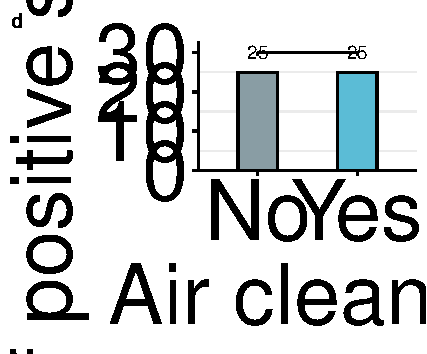
\includegraphics{../../results/mol-data/saliva-by-study-condition.pdf}\hspace{.5cm}
    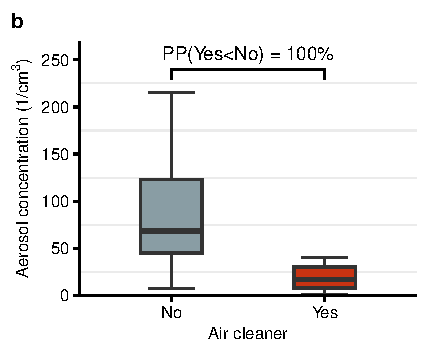
\includegraphics{../../results/env-data/aerosol-number-boxplot.pdf}
    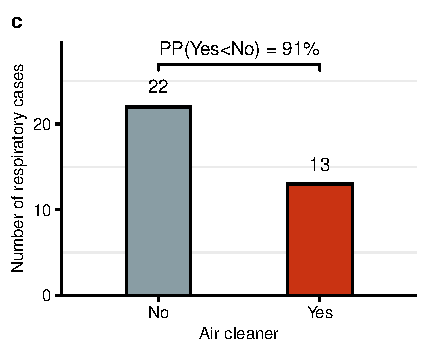
\includegraphics{../../results/epi-data/cases_by_condition.pdf}\hspace{.5cm}
    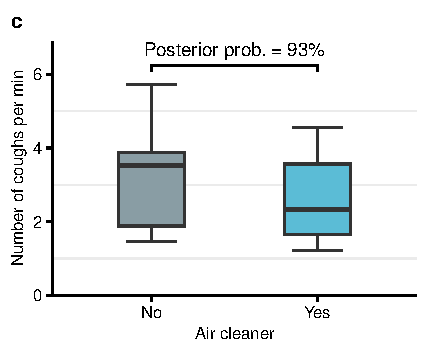
\includegraphics{../../results/cough-data/coughs-frequency-by-condition.pdf}
    \caption{\textbf{Risk of infection by study condition}. \textbf{(a)}~Number of positive saliva samples. \textbf{(b)}~Daily average aerosol number concentrations as boxplots. \textbf{(c)}~Number of respiratory cases. \textbf{(d)}~Daily average number of detected coughs per minute. The posterior probability (PP) for each outcome being lower with air cleaners (Yes<No) was computed based on the posterior samples of each Bayesian model used to estimate the effect of air cleaners after adjusting for confounders.}
    \label{fig:infection-risk}
\end{figure}

\FloatBarrier

\newpage

\section{Discussion}

% summary

We used a multiple-measurement approach to estimate the risk of respiratory virus infection in a Swiss school and assessed the effectiveness of air cleaners. We found a wide range of respiratory viruses in human saliva samples, mainly adenovirus, influenza B, and rhinovirus, but very few respiratory viruses were detected in bioaerosol samples and on the filters of the air cleaners. Aerosol number and particle mass concentrations decreased significantly with air cleaners and Bayesian modeling based on epidemiological data showed a potential reduction in the relative risk of infection with air cleaners. Reduced coughing could indicate that air cleaners prevent some symptomatic infections.

% comparison with previous study 

In a previous study\cite{Banholzer2023PLoSMed}, we estimated the effectiveness of mask wearing and air cleaners during winter 2022. Our previous study was conducted during the SARS-CoV-2 Omicron wave and most detected viruses were SARS-CoV-2. We found a detectable effect on the risk of SARS-CoV-2 infection only for mask wearing, but not air cleaners. We argued that air cleaners may have had less potential to reduce infections because they were introduced at the end of the study, when most students were already infected with SARS-CoV-2. In this study, we used a cross-over design and estimated the effectiveness of air cleaners during winter 2023. This time, we detected a range of respiratory viruses, which consisted primarily of adenovirus, influenza~B and rhinovirus, with only three positive SARS-CoV-2 saliva samples. A similar shift in the pattern of respiratory viruses has been observed in other studies\cite{Nygaard2023Lancet,Sauteur2022EuroSurv}. In contrast to our previous study, we found a small, potential benefit of air cleaners on the risk of respiratory infection. 

% discussing the effect of air cleaners

There may be several reasons for the relatively small effect of air cleaners. Compared to \eg universal mask wearing, which has been shown to be effective\cite{Banholzer2023PLoSMed,Heinsohn2022,Gettings2021,Leung2020NatMed,Milton2013PLoSPathogens}, air cleaners cannot affect transmission outside the classroom. Furthermore, previous work suggests that prolonged close contact may be necessary for transmission\cite{Leung2020NatMed,Brankston2007LancetID}, or make transmission more likely despite prior vaccination or infection\cite{Lind2023NatCommun}. However, compared to face masks, air cleaners are not able to prevent transmission by close range, high particle density. Evidence from our previous\cite{Banholzer2023PLoSMed} and this study further suggest that air cleaners are more effective at removing larger particles ($>5\mu$m). However, a greater proportion of respiratory viruses are carried in the smaller particles, which are also more relevant for transmission ($\leq5\mu$m)\cite{Fennelly2020}. Finally, classroom activity, airflow and other unobserved, confounding factors make it difficult to evaluate the effects of air cleaners. Nevertheless, it is important to assess their effectiveness in a real-world setting and to compare them with the hypothetical impact suggested by simulation studies\cite{Lindsley2021,Cortellessa2023Build}.

% economic and psychological impact of air cleaners
% tbd
% psychological part from Tina

% transmission within classroom

We detected only few respiratory viruses in bioaerosol samples (1~sample of adenovirus and 1~sample of rhinovirus ) and on the filters of the air cleaners (4~positive samples in 160~swabs) in this study. The low rate of positive bioaerosol samples means that it is unclear to what extent airborne transmission occurred in classrooms. It may be possible that students had relatively little exposure to respiratory viruses in schools and acquired their infections elsewhere. However, the distribution of saliva samples between classes shows remarkable differences. For example, adenovirus spread entirely in class~A during the first three study weeks and only two infections with influenza~B occurred over the study. In contrast, influenza~B spread throughout the study in class~B, and adenovirus infections were detected only in the last week of the study. Adenovirus infections tend to be mild\cite{Kunz2010CIDR} and less associated with cough than influenza\cite{Ma2018RMV}, which is consistent with the comparatively lower frequency of detected coughs in class~B. Taken together, the class-specific, spatiotemporal patterns in the spread of respiratory viruses indicate that transmission of respiratory infections may have occurred at least to some extent within the classrooms. 


% limitations

Our study has several limitations. First, aerosol measurements and molecular detection of viruses in bioaerosol samples document exposure, but not necessarily transmission and the direction of transmission (person to air, air to person) cannot be determined. However, the virus-specific distribution of positive saliva samples between classes (spatiotemporal pattern) may indicate transmission within classrooms. Second, the specific causes for the absences could not be determined from the epidemiological data. Therefore, some absences may have falsely been attributed to respiratory infections and we could only approximate the incubation period for each epidemiological case. Third, the effectiveness of air cleaners was somewhat limited because students occasionally had lessons outside the classroom. This is in contrast to other infection control measures such as face masks, which had to be used in every indoor space during the pandemic.

% conclusion

In conclusion, using epidemiological, environmental, and molecular data, our study showed that a wide range of non-SARS-CoV-2, but rarely SARS-CoV-2, was detected in students under non-pandemic conditions when public health measures were lifted, and that transmission of these respiratory viruses likely occurred in schools. Airborne detection of non-SARS-CoV-2 respiratory viruses was rare, suggesting that prolonged close contact may be required for transmission. Comparison with previous work during the pandemic, which showed frequent airborne SARS-CoV-2, suggests that respiratory viruses other than SARS-CoV-2 may be less detectable in the air. Air cleaners improved air quality by significantly reducing aerosol and particle concentrations. Based on our transmission model using epidemiological data, the risk of infection tends to be lower with air filters. Future studies should investigate the relative importance of prolonged close contact and long-range transmission of respiratory viruses in schools and other congregate settings.

\newpage

%TC:ignore

\section*{Funding}
This study is funded by the Multidisciplinary Center for Infectious Diseases, University of Bern, Bern, Switzerland. NB, LF, and ME are supported by the National Institute of Allergy and Infectious Diseases (NIAID) through cooperative agreement 5U01-AI069924-05. ME is supported by special project funding from the Swiss National Science Foundation (grant 32FP30-189498). \medskip

\section*{Author contributions}
Conception and design: NB, KZ, LF, PB, PJ, TS. Epidemiological and environmental data collection: NB, PJ, KZ, TS, LF. Laboratory data collection: PB, LFu. Additional data collection: TH. Cough detection: SB. Molecular genotyping: RD, AR, PB, LFu. Statistical analysis: NB. Paper draft: NB, LF, ME. All authors reviewed and approved the final version of the manuscript.


\section*{Acknowledgements}
We would like to thank the schools, teachers, and students participating in the study. We are grateful to the Educational Department of the canton of Solothurn for their support throughout the study. We also would like to thank the biosecurity team at the Institute for Infectious Diseases of the University of Bern for their assistance with the bioaerosol devices (Julia Feldmann, Monika Gsell, Kathrina Summermatter). Finally, we are indebted to the student assistants (Khadija Ahmed, Marie-Joséphine Brancato, Michelle Bürki, Santiago Martinez, Moric Toszeghi, Sylvain Wasmer) who helped with the data collection in the schools.

\bibliography{references.bib}
%TC:endignore

\end{document}
